%\documentstyle[epsf,twocolumn]{jarticle}       %LaTeX2e仕様
%\documentclass[twocolumn]{jarticle}     %pLaTeX2e仕様(platex.exeの場合)
\documentclass[onecolumn]{ujarticle}     %pLaTeX2e仕様(uplatex.exeの場合)
%%%%%%%%%%%%%%%%%%%%%%%%%%%%%%%%%%%%%%%%%%%%%%%%%%%%%%%%%%%%%%
%%
%%  基本バージョン
%%
%%%%%%%%%%%%%%%%%%%%%%%%%%%%%%%%%%%%%%%%%%%%%%%%%%%%%%%%%%%%%%%%
\setlength{\topmargin}{-45pt}
%\setlength{\oddsidemargin}{0cm} 
\setlength{\oddsidemargin}{-7.5mm}
%\setlength{\evensidemargin}{0cm} 
\setlength{\textheight}{24.1cm}
%setlength{\textheight}{25cm} 
\setlength{\textwidth}{17.4cm}
%\setlength{\textwidth}{172mm} 
\setlength{\columnsep}{11mm}

%\kanjiskip=.07zw plus.5pt minus.5pt


% 【節が変わるごとに (1.1)(1.2) … (2.1)(2.2) と数式番号をつけるとき】
%\makeatletter
%\renewcommand{\theequation}{%
%\thesection.\arabic{equation}} %\@addtoreset{equation}{section}
%\makeatother

%\renewcommand{\arraystretch}{0.95} 行間の設定
%%%%%%%%%%%%%%%%%%%%%%%%%%%%%%%%%%%%%%%%%%%%%%%%%%%%%%%%
%\usepackage{graphicx}   %pLaTeX2e仕様(\documentstyle ->\documentclass)
\usepackage[dvipdfmx]{graphicx}
\usepackage{subcaption}
\usepackage{multirow}
%%%%%%%%%%%%%%%%%%%%%%%%%%%%%%%%%%%%%%%%%%%%%%%%%%%%%%%%
\begin{document}
	
	%bibtex用の設定
	%\bibliographystyle{ujarticle} 
	
	\noindent
	
	\hspace{1em}
	2019 年 5 月 10 日
	ゼミ資料
	\hfill
	M1 寺内 光
	
	\vspace{2mm}
	
	\hrule
	
	\begin{center}
		{\Large \bf 進捗報告}
	\end{center}
	
	
	\hrule
	\vspace{3mm}
	
	% ‚ここから 文章 Start!
	\section{目のみ画像の識別,分散表現}
	目抜きの画像の識別と比べるために,目のみの画像を用いて識別タスクを行い,その分散表現をプロットした.また,目のパーツが入っていない画像は除去して実験を行ったため,各タッチの枚数が異なる.
	
	表 \ref{tab:num_image} に各タッチの画像枚数を示す.
	\begin{table}[h]
		\centering
		\caption{目のみデータセットの各タッチ枚数}
		\begin{tabular}{|c|c|} \hline
			萌えタッチ&64\\ \hline
			青年漫画タッチ&74\\ \hline
			少年漫画タッチ&66\\ \hline
		\end{tabular}
		\label{tab:num_image}
	\end{table}

	表 \ref{tab:accuracy} に各タッチのテスト識別率を示す.
	\begin{table}[h]
		\centering
		\caption{目のみ画像のテスト識別率}
		\begin{tabular}{|c|c|} \hline
			識別器&accuracy\\ \hline
			CAE + RF&0.821\\ \hline
			CAE + SVM&0.718\\ \hline
			AE + RF&0.436\\ \hline
			AE + SVM&0.333\\ \hline
		\end{tabular}
		\label{tab:accuracy}
	\end{table}

	目のみになると AE よりも CAE のほうがさらに有効であることが確認できた.
	
	表 \ref{tab:etc} に各タッチの混同行列を示す.
	\begin{table}[h]
		\begin{center}
			\caption{混同行列}
			\label{tab:etc}
			\vspace{-4mm}
			\begin{tabular}{|c|c||c|c|c|}\hline
				\multicolumn{2}{|c||}{}&\multicolumn{3}{|c|}{予測値} \\ \cline{3-5}
				\multicolumn{2}{|c||}{}&萌え&青年&少年 \\ \hline \hline
				\multirow{2}{*}{真}&萌え&9&0&0\\ \cline{2-5}
				\multirow{2}{*}{値}&青年&0&14&3\\ \cline{2-5}
				&少年&0&4&9\\ \hline
			\end{tabular}
		\end{center}
	\end{table}
	
	図 \ref{fig:tsne} に目の分散表現を t-SNE でプロットした結果を示す.
	\begin{figure}[h]
		\begin{center}
			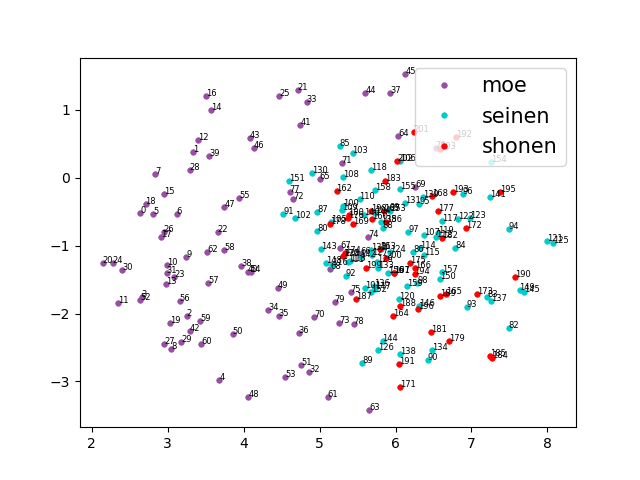
\includegraphics[width=0.8\columnwidth]{t_sne_CAE_hwf_80_weight_all.png}
			\caption{目のみ画像の t-SNE 結果}
			\label{fig:tsne}
		\end{center}
	\end{figure}
	萌えタッチの目の特徴が他とは異なることが見て取れる.
	
	図 \ref{fig:touch_example} に各タッチの目の例を示す.
	\begin{figure}[t]
		\vspace{-4mm}
		\centering
		\begin{subfigure}{0.49\columnwidth}
			\centering
			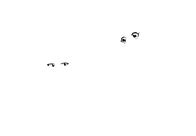
\includegraphics[width=1.2\columnwidth]{eye_shonen.png}
			\caption{少年漫画タッチ}
			\label{fig:shonen}
		\end{subfigure}
		\begin{subfigure}{0.49\columnwidth}
			\centering
			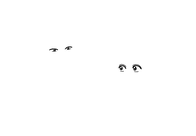
\includegraphics[width=1.2\columnwidth]{eye_seinen.png}
			\caption{青年漫画タッチ}
			\label{fig:seinen}
		\end{subfigure}
		\begin{subfigure}{0.49\columnwidth}
			\centering
			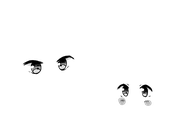
\includegraphics[width=1.2\columnwidth]{eye_moe.png}
			\caption{萌えタッチ}
			\label{fig:moe}
		\end{subfigure}
		\caption{各タッチ例}
		\label{fig:touch_example}
	\end{figure}

	\section{PFNインターン コーディング課題終了}
	貴重な GW を全部奪われたが無事に完成.

	\section{来週以降の予定}
	\begin{itemize}
		\item JSAIおよび前期研究発表会のスライド準備
		\item manpu?
		\item パーツ抜き画像の学習モデルを作る
	\end{itemize}
	
\end{document}